\chapter{Introduction}

\textcolor{green}{Jo: quote is fine, but better Sth Like : Mark Weiser once
wrote in his visionary paper from whenever [22]:}

\begin{quote}
\emph{``The most profound technologies are those that disappear. They weave
themselves into the fabric of everyday life until they are indistinguishable
from it''} 
Mark Weiser \cite{Weiser_ComputerIn21stCentury}
\end{quote}


\textcolor{blue}{some intro words here.. .. and later stuff about .. The chapter
begins with an introduction to wireless sensor nodes and Wireless Sensor Networks (WSNs). This is followed by a
description of the protocol stack used in this work}



\section{Introduction to Wireless Sensor Networks}

Recent advances in micro system technologies and wireless communication
made it possible to deploy wireless sensor networks (WSNs) that contain a large
number of sensor nodes, multifunctional devices characterised by their low- cost,
low-power, and small form factor, that can communicate across short distances
using Radio Frequency (RF) communication \cite{SensorSurveyAkyildiz:2002}.

WSNs are being used in a wide range of applications in military and civilian
operations such as, for instance, health monitoring, environment monitoring,
data acquisition in dangerous environments, and target tracking.

This chapter begins with the introduction of sensor nodes and
discussion over followed by presentation of the most important features of WSNs.

\subsection{Sensor Nodes} \label{subsec:sensornodes}

Typically, a sensor node consists of the following elemants (as it can be seen
from the Figure \ref{Fig:SensorNodeArch})
\begin{itemize}
  \item \emph{Sensing unit}, which is comprised of a number of sensors and
  analog-to-digital converters. 
  \item \emph{Tranceiver}, which facilitates node-node communication using 
a variety of techniques.
  \item \emph{Processing unit}, that usually comprises a 
microcontroller/microprocessor that performs processing, and is associated with 
a storage unit.
  \item \emph{Power unit}, which provides the energy required to run the sensor node, and can use chemical 
batteries or power scavenging units such as solar cells.
\end{itemize}


\begin{figure}
\centering
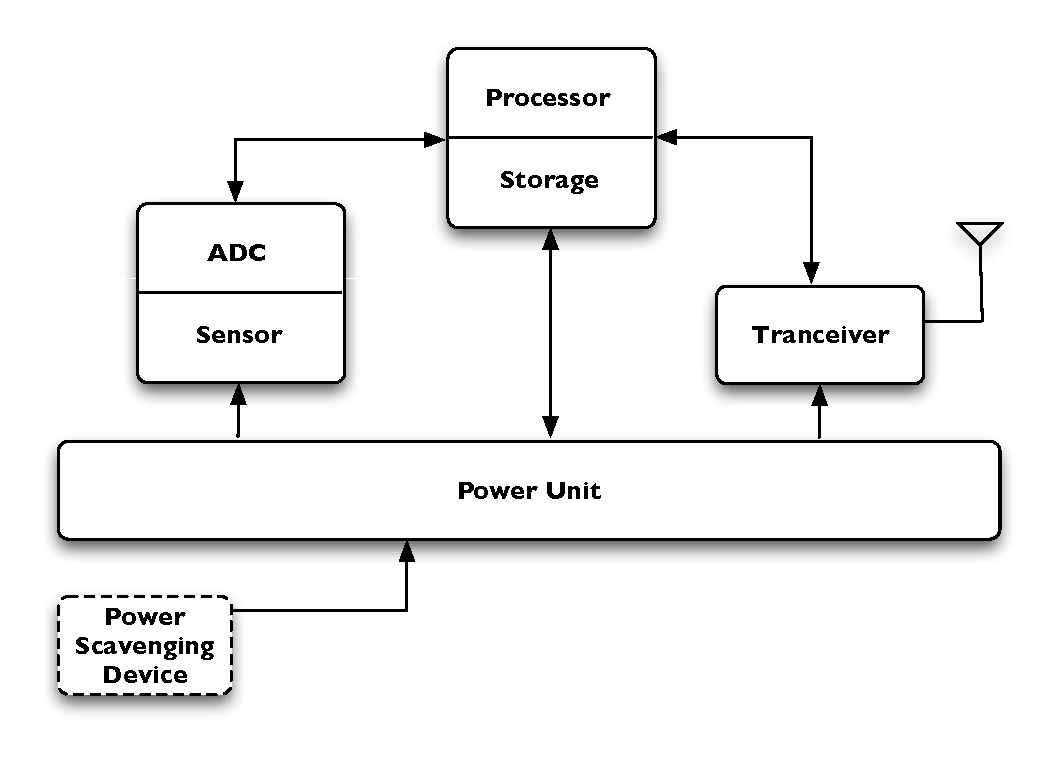
\includegraphics[scale=0.65]{img/SensorNodeArch.eps} 
\caption[Architecture of a sensor node] {Architecture of a sensor node (adapted from \cite{SensorSurveyAkyildiz:2002}).}
\label{Fig:SensorNodeArch}
\end{figure} 


\textcolor{green}{the next paragraph needs a bit of reformulation. about the constraints
I think your argumentation should go like size/weight -> battery  (that's the
point where it really gets hard to make smaller). -> energy efficient processing, memory and so on
and cost as an additional constraint }

Sensor nodes have constraints on both their size and their cost. The former 
constraint arises from the requirement that sensor nodes be easily deployable, 
while the latter arises from the requirement for fault tolerance (which in turn 
can be achieved only by being able to deploy cost-effectively large numbers of
sensor nodes in the environment being monitored). These limit the memory capacity, processing 
power, and the amount of energy available on a particular node.

\subsection{Wireless Sensor Networks}
\textcolor{green}{the first sentence of 2.1.2 is a bit well, almost German
too long and self referring. actually, what you write about in that section, is more like routing in networks of sensor nodes
maybe you should expand a bit}

As mentioned in the previous section, sensor nodes are capable of communicating
untethered with one another, and hence are capable of forming networks of nodes
called a Wireless Sensor Network. 

WSNs are typically deployed randomly in an
environment where phenomena are required to be monitored. 

A WSN is self-organising system, given the random nature of the deployment.

Its topology is subject to change, and therefore sensor nodes should be
capable of dealing with changes of this kind in order to cope with hostile
operating conditions, the failure-prone nature of sensor nodes and the possibility of 
redeployment of additional sensor nodes at any time during operation.


\section{WSN Protocol Stack} \label{sec:WSNProtStack}

The WSN protocol stack presented in \cite{SensorSurveyAkyildiz:2002} is adapted
from \cite{ComputerNetworksTannenbaum:2003}. As it can be seen from the
Figure \ref{Fig:ProtStack}, the WSN protocol stack consists of the following layers:

\begin{itemize}
\item \emph{Physical Layer}, which provides the transmission of data over the physical transmission medium.
\item \emph{Data Link Layer}, which deals with power-aware Medium Access Control (MAC) protocols that minimise collisions and transceiver on-time.
\item \emph{Network Layer}, which is primarily responsible for
routing data across the network.
\item \emph{Transport Layer}, which provides reliable delivering of data and
supports error checking mechanisms.
\item \emph{Application Layer}, where the application software is resided.
\end{itemize}

\begin{figure}
\centering
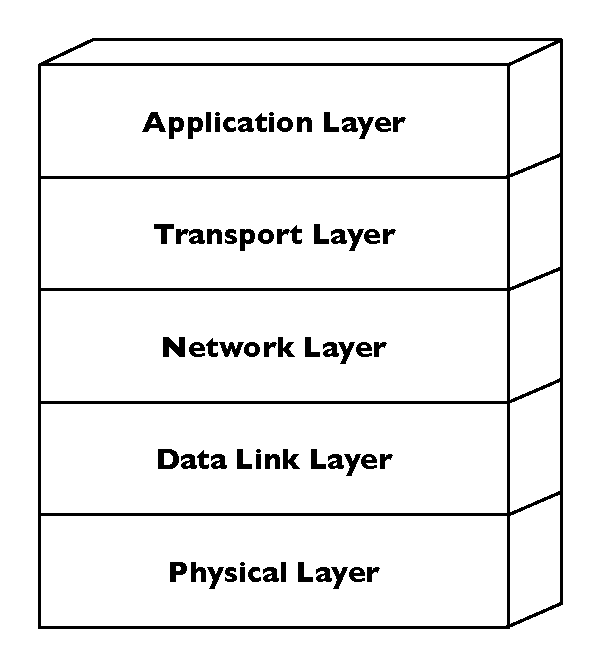
\includegraphics[scale=0.65]{img/ProtStack.eps}
\caption[WSN protocol stack]{WSN protocol stack (reproduced from \cite{SensorSurveyAkyildiz:2002})}
\label{Fig:ProtStack}
\end{figure}
